\section{Linear Maps}

We'll present linear maps with different definitions, one more practical, one geometric and finally the more abstract definition.

Practically, matrices are the coordinate version of linear maps. If you represent vectors as column, covectors as row vectors, linear maps are
represented by matrices.
How do matrices act on vectors? Let's see a simple example:

\begin{equation}
    \begingroup\color{red}\begin{bmatrix}
        3 & 4\\
        -1 & 2
    \end{bmatrix}\endgroup \begin{bmatrix}
        2\\
        1
    \end{bmatrix} = \begin{bmatrix}
        2\\
        0
    \end{bmatrix}
\end{equation}

What is actually doing? 
If we test using a "copy" of the basis vectors $\vec{e_1}, \vec{e_2}$, we see that the outputs are
respectively, the first and second column of the matrix:

\begin{equation}
    \begin{bmatrix}
        \begingroup\color{red}3\endgroup & 4\\
        \begingroup\color{red}-1\endgroup & 2
    \end{bmatrix} \begin{bmatrix}
        1\\
        0
    \end{bmatrix} = \begin{bmatrix}
        \begingroup\color{red}3\endgroup\\
        \begingroup\color{red}-1\endgroup
    \end{bmatrix}
\end{equation}

\begin{equation}
    \begin{bmatrix}
        3 & \begingroup\color{red}4\endgroup\\
        -1 & \begingroup\color{red}2\endgroup
    \end{bmatrix} \begin{bmatrix}
        0\\
        1
    \end{bmatrix} = \begin{bmatrix}
        \begingroup\color{red}4\endgroup\\
        \begingroup\color{red}2\endgroup
    \end{bmatrix}
\end{equation}

\textbf{Why do we stress about these being copies of basis vectors? Because Linear Maps tranform 
input vectors, they do not transform the basis.}
The $i^{th}$ column of the matrix is the image of the $i^{th}$ copy of the basis vector.

Geometrically, linear maps are spatial transforms that:
\begin{itemize}
    \item Keep gridlines parallel
    \item Keep gridlines evenly spaced
    \item Keep the origin stationary
\end{itemize}

And abstractly, linear maps are maps from a vector space to another:

\begin{equation}
    \textit{L}:\textit{V} \to \textit{W}
\end{equation}

And obey linearity rules:

\begin{align*}
    \textit{L}\left(\vec{v} + \vec{w}\right) &= \textit{L}\left(\vec{v}\right) + \textit{L}\left(\vec{w}\right)\\
    \textit{L}\left(n\vec{v}\right) &= n\textit{L}\left(\vec{v}\right)
\end{align*}

Now let's see how the abstract and coordinate definitions are related to each other. Let's review the formula for matrix multiplication of a 2x2 matrix:

\begin{equation}
    \begin{bmatrix}
        a & b\\
        c & d
    \end{bmatrix} \begin{bmatrix}
        \begingroup\color{red}x\endgroup\\
        \begingroup\color{blue}y\endgroup
    \end{bmatrix} = 
        \begin{bmatrix}
            a\begingroup\color{red}x\endgroup + b\begingroup\color{blue}y\endgroup\\
            c\begingroup\color{red}x\endgroup + d\begingroup\color{blue}y\endgroup
        \end{bmatrix}
\end{equation}

At a first glance, this rule may come out from nowhere, but this is actually a direct consequence of the abstract definition above.
To show this, let's start by saying that we have a linear map $\textit{L}:\textit{V} \to \textit{V}$ acting on a vector $\vec{v}$ to produce some output vector $\vec{w}$.
\textbf{The assumption to stay in the same vector space is needed to ensure we can use the same basis vectors on both inputs and outputs}:

\begin{align*}
    \begingroup\color{violet}\vec{w}\endgroup &= 
    \textit{L}\left(\begingroup\color{orange}\vec{v}\endgroup\right) = 
    \textit{L}\left(\begingroup\color{orange}v^1\endgroup\begingroup\color{blue}\vec{e_1}\endgroup + 
    \begingroup\color{orange}v^2\endgroup\begingroup\color{blue}\vec{e_2}\endgroup\right)\\
    &= \begingroup\color{orange}v^1\endgroup\textit{L}\left(\begingroup\color{blue}\vec{e_1}\endgroup\right) + \begingroup\color{orange}v^2\endgroup\textit{L}\left(\begingroup\color{blue}\vec{e_2}\endgroup\right)
\end{align*}

These $\textit{L}\left(\begingroup\color{blue}\vec{e_1}\endgroup\right)$ and $\textit{L}\left(\begingroup\color{blue}\vec{e_2}\endgroup\right)$ are
just vectors in $\textit{V}$ so we can write them down in terms of the basis vectors:

\begin{align*}
    \textit{L}\left(\begingroup\color{blue}\vec{e_1}\endgroup\right) &= \textit{L}^1_1\begingroup\color{blue}\vec{e_1}\endgroup + \textit{L}^2_1\begingroup\color{blue}\vec{e_2}\endgroup\\
    \textit{L}\left(\begingroup\color{blue}\vec{e_2}\endgroup\right) &= \textit{L}^1_2\begingroup\color{blue}\vec{e_1}\endgroup + \textit{L}^2_2\begingroup\color{blue}\vec{e_2}\endgroup
\end{align*}

\begin{align*}
    \begingroup\color{violet}\vec{w}\endgroup &= \begingroup\color{orange}v^1\endgroup\left(\textit{L}^1_1\begingroup\color{blue}\vec{e_1}\endgroup + \textit{L}^2_1\begingroup\color{blue}\vec{e_2}\endgroup\right) + \begingroup\color{orange}v^2\endgroup\left(\textit{L}^1_2\begingroup\color{blue}\vec{e_1}\endgroup + \textit{L}^2_2\begingroup\color{blue}\vec{e_2}\endgroup\right)\\
    &= \left(\textit{L}^1_1\begingroup\color{orange}v^1\endgroup + \textit{L}^1_2\begingroup\color{orange}v^2\endgroup\right) \begingroup\color{blue}\vec{e_1}\endgroup + \left(\textit{L}^2_1\begingroup\color{orange}v^1\endgroup + \textit{L}^2_2\begingroup\color{orange}v^2\endgroup\right) \begingroup\color{blue}\vec{e_2}\endgroup\\
    &= \begingroup\color{violet}w^1\endgroup\begingroup\color{blue}\vec{e_1}\endgroup + \begingroup\color{violet}w^2\endgroup\begingroup\color{blue}\vec{e_2}\endgroup
\end{align*}

So we've derived how to transform the $v$ coefficients into the $w$ coefficients.

\begin{align*}
    \begingroup\color{violet}w^1\endgroup &= \textit{L}^1_1\begingroup\color{orange}v^1\endgroup + \textit{L}^1_2\begingroup\color{orange}v^2\endgroup\\
    \begingroup\color{violet}w^2\endgroup &= \textit{L}^2_1\begingroup\color{orange}v^1\endgroup + \textit{L}^2_2\begingroup\color{orange}v^2\endgroup
\end{align*}

which are nothing more than the usual 2x2 matrix multiplication rule:

\begin{equation}
    \begin{bmatrix}
        L^1_1 & L^1_2\\
        L^2_1c & L^2_2
    \end{bmatrix} \begin{bmatrix}
        \begingroup\color{orange}v^1\endgroup\\
        \begingroup\color{orange}v^2\endgroup
    \end{bmatrix} = 
        \begin{bmatrix}
            \begingroup\color{violet}w^1\endgroup\\
            \begingroup\color{violet}w^2\endgroup
        \end{bmatrix}
\end{equation}

For any number of dimensions, we can write:

\begin{equation}
    \begingroup\color{violet}\vec{w}\endgroup = \textit{L}\left(\begingroup\color{orange}\vec{v}\endgroup\right) = \sum_{i=1}^{n}\begingroup\color{violet}w^i\endgroup\begingroup\color{blue}\vec{e_i}\endgroup
\end{equation}

And the linear maps coefficients:

\begin{equation} \label{eq:linear-map-transform}
    \textit{L}\left(\begingroup\color{blue}\vec{e_i}\endgroup\right) = \sum_{j=1}^{n}\textit{L}^j_i\begingroup\color{blue}\vec{e_j}\endgroup
\end{equation}

And we can transform finally, the $v$ components into $w$ components:

\begin{equation}
    \begingroup\color{violet}w^i\endgroup = \sum_{j=1}^{n}\textit{L}^i_j\begingroup\color{orange}v^j\endgroup
\end{equation}

which is indeed the matrix multiplication formula applied to n-dimension space.

We can now proceed checking how linear maps transform when moving from one basis to another.

\begin{center}
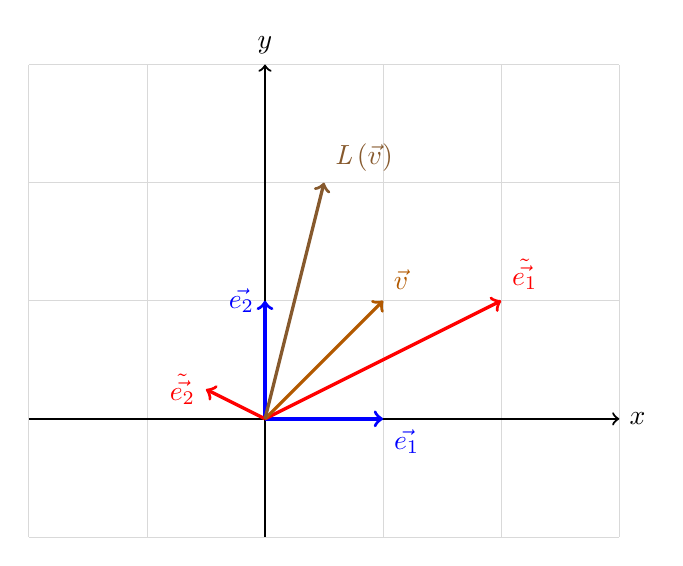
\begin{tikzpicture}[scale=1.5]
  \draw[step=1cm,gray!30,very thin] (-2,-1) grid (3,3);
  \draw[->,thick] (-2,0) -- (3,0) node[right] {$x$};
  \draw[->,thick] (0,-1) -- (0,3) node[above] {$y$};

  % Old basis (blue)
  \draw[->,very thick,blue] (0,0) -- (1,0) node[below right] {$\vec{e_1}$};
  \draw[->,very thick,blue] (0,0) -- (0,1) node[left] {$\vec{e_2}$};

  % New basis (red)
  \draw[->,very thick,red] (0,0) -- (2,1) node[above right] {$\tilde{\vec{e_1}}$};
  \draw[->,very thick,red] (0,0) -- (-0.5,0.25) node[left] {$\tilde{\vec{e_2}}$};

  % Vector v (orange)
  \draw[->,very thick,orange!70!black] (0,0) -- (1,1) node[above right] {$\vec{v}$};

  % Linear map (brown)
  \draw[->,very thick,brown!70!black] (0,0) -- (0.5,2) node[above right] {$\textit{L}\left(\vec{v}\right)$};
\end{tikzpicture}

\end{center}

Consider the diagram above and the linear map expressed by the matrix in the $\color{blue}\vec{e_i}$ basis:

\begin{equation}
    \begin{bmatrix}
        1/2 & 0\\
        0 & 2
    \end{bmatrix}_{\color{blue}\vec{e_i}}
\end{equation}

As reminder, this means that:

\begin{align*}
    \textit{L}\left(\begingroup\color{blue}\vec{e_1}\endgroup\right) &= 1/2\begingroup\color{blue}\vec{e_1}\endgroup \\
    \textit{L}\left(\begingroup\color{blue}\vec{e_2}\endgroup\right) &= 2\begingroup\color{blue}\vec{e_2}\endgroup
\end{align*}

Vector $\color{orange}\vec{v}$ has components $1, 1$ in the basis $\color{blue}\vec{e_i}$.
So what would be the components of the vector $\textit{L}\left(\begingroup\color{orange}\vec{v}\endgroup\right)$ ?

\begin{equation}
    \textit{L}\left(
        \begin{bmatrix}
            1\\
            1
        \end{bmatrix}_{\color{blue}\vec{e_i}}
    \right) = 
    \begin{bmatrix}
        \begingroup\color{brown}1/2\endgroup\\
        \begingroup\color{brown}2\endgroup
    \end{bmatrix}_{\color{blue}\vec{e_i}}
\end{equation}

Remember that, if we apply the backward transformation to these vector components, we 
obtain the vector components in the new basis $\color{red}\tilde{\vec{e_i}}$:

\begin{equation}
    \begin{bmatrix}
        1/4 & 1/2\\
        -1 & 2
    \end{bmatrix}\begin{bmatrix}
        \begingroup\color{orange}1\endgroup\\
        \begingroup\color{orange}1\endgroup
    \end{bmatrix}_{\color{blue}\vec{e_i}} = 
    \begin{bmatrix}
        \begingroup\color{orange}3/4\endgroup\\
        \begingroup\color{orange}1\endgroup\\
    \end{bmatrix}_{\color{red}\tilde{\vec{e_i}}}
\end{equation}

So, the next question might be, what are the components of the linear map output vector
in the new basis?

\begin{equation}
    \textit{L}\left(
        \begin{bmatrix}
            \begingroup\color{orange}3/4\endgroup\\
            \begingroup\color{orange}1\endgroup\\
        \end{bmatrix}_{\color{red}\tilde{\vec{e_i}}}
    \right) = 
    \begin{bmatrix}
        \begingroup\color{brown}?\endgroup\\
        \begingroup\color{brown}?\endgroup
    \end{bmatrix}_{\color{red}\tilde{\vec{e_i}}}
\end{equation}

We cannot use the matrix representation we used before, because that's tied to the 
old basis vectors, so what we need to do is finding a new matrix that represents
the linear map in the new basis, which means we need to find these coefficients:

\begin{align*}
    \textit{L}\left(\begingroup\color{red}\tilde{\vec{e_1}}\endgroup\right) &= \tilde{L}^1_1\begingroup\color{red}\tilde{\vec{e_1}}\endgroup + \tilde{L}^2_1\begingroup\color{red}\tilde{\vec{e_2}}\endgroup\\
    \textit{L}\left(\begingroup\color{red}\tilde{\vec{e_2}}\endgroup\right) &= \tilde{L}^1_2\begingroup\color{red}\tilde{\vec{e_1}}\endgroup + \tilde{L}^2_2\begingroup\color{red}\tilde{\vec{e_2}}\endgroup
\end{align*}

\begin{equation}
    \sum_{q=1}^{n}\tilde{L}^q_i\begingroup\color{red}\tilde{\vec{e_q}}\endgroup = L\left(\begingroup\color{red}\tilde{\vec{e_i}}\endgroup\right)
\end{equation}

We can use the forward transform to re-write the new basis vectors in terms of the old ones:

\begin{align*}
    \sum_{q=1}^{n}\tilde{L}^q_i\begingroup\color{red}\tilde{\vec{e_q}}\endgroup &= L\left(\sum_{j=1}^{n} F^j_i \begingroup\color{blue}\vec{e_j}\endgroup\right)\\
    &= \sum_{j=1}^{n} F^j_i L\left(\begingroup\color{blue}\vec{e_j}\endgroup\right)
\end{align*}

Now we can use the formula that expresses the linear map output as linear combinaton of the old basis vectors (\ref{eq:linear-map-transform}) and re-arranging:

\begin{align*}
    \sum_{q=1}^{n}\tilde{L}^q_i\begingroup\color{red}\tilde{\vec{e_q}}\endgroup &= \sum_{j=1}^{n} F^j_i \sum_{k=1}^{n}\textit{L}^k_j\begingroup\color{blue}\vec{e_k}\endgroup\\
    &= \sum_{j=1}^{n}\sum_{k=1}^{n} F^j_i \textit{L}^k_j\begingroup\color{blue}\vec{e_k}\endgroup
\end{align*}

We can proceed re-writing the old basis vector in terms of the new one, using the backward transformation \ref{eq:backward}:

\begin{align*}
    \sum_{q=1}^{n}\tilde{L}^q_i\begingroup\color{red}\tilde{\vec{e_q}}\endgroup 
    &= \sum_{j=1}^{n}\sum_{k=1}^{n} F^j_i \textit{L}^k_j \sum_{l=1}^{n} B^l_k\begingroup\color{red}\tilde{\vec{e_l}}\endgroup\\
    &= \sum_{l=1}^{n}\sum_{j=1}^{n}\sum_{k=1}^{n} B^l_k \textit{L}^k_j F^j_i \begingroup\color{red}\tilde{\vec{e_l}}\endgroup
\end{align*}

Since the letter we use for the summation does not really matter, we can just rename all the q to l and we get:

\begin{align*}
    \sum_{l=1}^{n}\tilde{L}^l_i\begingroup\color{red}\tilde{\vec{e_l}}\endgroup 
    &= \sum_{l=1}^{n}\sum_{j=1}^{n}\sum_{k=1}^{n} B^l_k \textit{L}^k_j F^j_i \begingroup\color{red}\tilde{\vec{e_l}}\endgroup
\end{align*}

Finally, we see that the $\tilde{L}$ coefficients are obtained by multiplying the backward transform on the left, and forward transform on the right, of the old coefficients:

\begin{subequations}
\begin{empheq}[box=\widefbox]{align}
    \tilde{L}^l_i = \sum_{j=1}^{n}\sum_{k=1}^{n}B^l_k L^k_j F^j_i
\end{empheq}
\end{subequations}

You can think about this, the $\widetilde{L}$ transformation takes us from the input vector components to the output vector components in the new basis.
Instead of "travelling" along this "arrow" (bottom of diagram below), we move from the new vector componens to the new vector components using the forward transformation.
Then, to transform the components of the input vector to the components of the output vector, we apply the $\textit{L}$ transformation.
And finally, to get from the old vector components to the new ones, we apply the backward transformation $B$

\begin{center}
\begin{tikzpicture}[
    node distance=2.5cm,
    equation/.style={font=\large},
    arrow/.style={->, thick, >=stealth}
]

% Top left node
\node[equation] (topleft) {
    $L \left(\begin{bsmallmatrix} 1 \\ 1 \end{bsmallmatrix}_{\vec{e}_i}\right)$
};

% Top right node (just the result, positioned to the right)
\node[equation, right=3cm of topleft] (topright) {
    $\begin{bsmallmatrix} 1/2 \\ 2 \end{bsmallmatrix}_{\vec{e}_i}$
};

% Bottom right node
\node[equation, below=1.8cm of topright] (bottomright) {
    $\begin{bsmallmatrix} ? \\ ? \end{bsmallmatrix}_{\widetilde{\vec{e}}_i}$
};

% Bottom left node
\node[equation, left=3cm of bottomright] (bottomleft) {
    $L \left(\begin{bsmallmatrix} 3/4 \\ 1 \end{bsmallmatrix}_{\widetilde{\vec{e}}_i}\right)$
};

% Arrows connecting the cycle
% Top: L transformation (curved arrow from left to right over the equation)
\draw[arrow, bend left=30]
    ([yshift=0.2cm]topleft.north) to node[above] {$L$} ([yshift=0.2cm]topright.north);

% Right: change of basis (down arrow)
\draw[arrow]
    (topright) -- node[right] {$B$} (bottomright);

% Bottom: L~ transformation (curved arrow from right to left under the equation)
\draw[arrow, bend right=30]
    ([yshift=-0.2cm]bottomleft.south) to node[below] {$\widetilde{L}$} ([yshift=-0.2cm]bottomright.south);

% Left: F transformation (up arrow)
\draw[arrow]
    (bottomleft) -- node[left] {$F$} (topleft);

\end{tikzpicture}

\end{center}

Now you've noticed how heavy the derivation and notation, especially related to the 
summation involved, was above.
We will, from now on, adopt the Einstein summation convention, which states that, everytime indeces appear both at the bottom and at the top, a
summation is implicitly expected.

That means that in our case, of the linear map transformation:

\begin{subequations}
\begin{empheq}[box=\widefbox]{align}
    \tilde{L}^l_i = B^l_k L^k_j F^j_i
\end{empheq}
\end{subequations}

Because the repeating indeces, appearing at the top and bottom, are k and j, they're implicitly summed from 1 to n.
Using this trick now, we can try deriving the backward transformation, from the $\widetilde{L}$ to the direct linear map $\textit{L}$.

Let's take this equation, and what we want, is isolating the $L^k_j$ on the right side.
To do that, we need to take out those $B$ and $F$ maps on the right side.
How do we do this? We can consider that multiplying $F$ and $B$ together gives the identity matrix, so we can 
multiply by $F$ and $B$ on both sides of the equation:

\begin{align*}
    \tilde{L}^l_i &= B^l_k L^k_j F^j_i\\
    \begingroup\color{red}F^s_l\endgroup \tilde{L}^l_i \begingroup\color{blue}B^i_t\endgroup &=
    \begingroup\color{red}F^s_l\endgroup B^l_k L^k_j F^j_i \begingroup\color{blue}B^i_t\endgroup\\
    \begingroup\color{red}F^s_l\endgroup \tilde{L}^l_i \begingroup\color{blue}B^i_t\endgroup &=
    \begingroup\color{red}\delta^{s}_k\endgroup L^k_j \begingroup\color{blue}\delta^{j}_t \endgroup\\
    \begingroup\color{red}F^s_l\endgroup \tilde{L}^l_i \begingroup\color{blue}B^i_t\endgroup &=
    \begingroup\color{red}\delta^{s}_k\endgroup L^k_t\\
    \begingroup\color{red}F^s_l\endgroup \tilde{L}^l_i \begingroup\color{blue}B^i_t\endgroup &=
    L^s_t
\end{align*}

So we obtain:

\begin{subequations}
\begin{empheq}[box=\widefbox]{align}
    \begingroup\color{red}F^s_l\endgroup \tilde{L}^l_i \begingroup\color{blue}B^i_t\endgroup &=
    L^s_t
\end{empheq}
\end{subequations}

